% main.tex
\documentclass{article}

\usepackage[pdfauthor={CoderDojo Linz},
            pdftitle={Äpfel sammeln}]
            {hyperref}

\newcommand{\footertitle}{Äpfel sammeln}
% settings.tex
\usepackage[
    a4paper, 
    top=2cm,
    left=1cm,
    right=1cm,
    bottom=2cm
]{geometry}

\usepackage{fontspec}
\usepackage{graphicx}
\usepackage{hyperref}
\usepackage{fancyhdr}
\usepackage[ngerman]{babel}
\usepackage{wrapfig}
\usepackage{enumitem}
\usepackage{titlesec} 
\usepackage{ragged2e}
\usepackage{tcolorbox}
\usepackage{array}
\usepackage[table]{xcolor}
\usepackage{fontawesome5}

\setmainfont{Carlito}

% Fancyhdr setup
\fancypagestyle{defaultpagestyle}{
    \fancyhf{} % Clear all headers and footers
    \fancyhead[C]{
\includegraphics[width=5cm]{../../CoderDojo_Logo.png}} 
    \renewcommand{\headrulewidth}{0pt} % Remove header line
    \renewcommand{\footrulewidth}{0pt} % Remove footer line
    \fancyfoot[L]{\footertitle}
    \fancyfoot[R]{Seite \thepage} % Right footer with page number
}

\newcommand{\SectionDesign}[4]{
    \noindent
    \csname #1*\endcsname{\textcolor[HTML]{1E90FF}{\fontsize{#2pt}{#3pt}\selectfont #4}}
}

\newcommand{\TextAndImage}[5][{}]{
    \fontsize{11pt}{16pt}\selectfont
    \noindent
    \begin{minipage}[c]{#4\textwidth}
    \RaggedRight
    #2 % First parameter: text
    \end{minipage}
    \hfill
    \begin{minipage}[c]{#5\textwidth}
    \includegraphics[width=\textwidth, #1]{#3} % Second parameter: image file name
    \end{minipage}
}

\newcommand{\ImageAndText}[2]{
    \fontsize{16pt}{24pt}\selectfont
    \noindent
    \begin{minipage}[c]{0.65\textwidth}
        \includegraphics[width=\textwidth]{#1} % Second parameter: image file name
    \end{minipage}
    \hfill % Fills the space between the minipages
    \begin{minipage}[c]{0.25\textwidth}
        \centering
        #2 % First parameter: text
    \end{minipage}
}

\newcommand{\TextDesign}[1]{
    \fontsize{11pt}{16pt}\selectfont
    \noindent
    \RaggedRight
    #1 % First parameter: text
}
\graphicspath{{images/}}

\begin{document}
    \pagestyle{defaultpagestyle}

    \SectionDesign{section}{24}{24}{\textbf{Äpfel sammeln}}
    \vspace{0.5cm}
     
    \ImageAndText{ÄpfelSammeln.png}{
    \centering
    In diesem Spiel sammelst du Äpfel, die auf einer Hecke platziert sind und von links nach rechts scrollen. Gleichzeitig musst du Vögeln ausweichen, die von rechts nach links fliegen.
    }{0.65}{0.25}{16}{24}

    \vspace{1cm}
    \SectionDesign{subsection}{18}{24}{\textbf{Ziel des Spieles}}
    \vspace{0.5cm}

    \TextDesign{
    Dein Ziel ist es, 25 Äpfel zu sammeln, um zu gewinnen. Wenn du einen Vogel berührst oder die ersten 10 Äpfel verpasst, verlierst du das Spiel. Die Herausforderung besteht darin, den richtigen Moment abzupassen, um Äpfel zu sammeln, ohne von den Vögeln getroffen zu werden. Viel Erfolg!
    }

    \vspace{1cm}
    \SectionDesign{subsection}{18}{24}{\textbf{Bühne und Figuren anlegen}}

    \vspace{0.5cm}
    \SectionDesign{subsubsection}{14}{24}{Spielfeld}
    \vspace{-1cm}
    
    \TextAndImage{
    \vspace{-0.5cm}
    Als erstes legst du fest, wie deine Bühne aussehen soll. Für dieses Spiel brauchst du einen blauen Himmel als Hintergrund. Wähle ein passendes Bild aus oder male selbst eines.}{Spielfeld.png}{0.45}{0.45}{11}{16}


    % NEW PAGE
    \newpage
    \vspace{0.5cm}
    \SectionDesign{subsubsection}{14}{24}{Figuren}
    \vspace{0.5cm}

    \TextAndImage{
    Als erste Figur brauchst du eine Person deiner Wahl (zum Beispiel die Figur \textit{Hannah}). Den Scratchy darfst du löschen. Du fügst es mit \textit{Figur wählen} ein. Außerdem brauchst du noch eine Hecke, einen Apfel, einen Vogel und einen Boden, die du entweder selbst mit Midjourney generieren, selber zeichnen oder aus den vorhandenen Figuren wählen kannst
    
    \vspace{\baselineskip}
    \textbf{\textcolor[HTML]{1E90FF}{Achtung:} Die Figuren Apfel und Vogel kannst du verstecken, indem du \textit{Sichtbarkeit} deaktivierst.}
    }{Figuren.png}{0.45}{0.45}{11}{16}

    \vspace{0.25cm}
    \RaggedLeft
    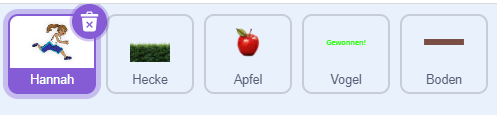
\includegraphics[width=10cm]{Figuren2.png}

    \vspace{0.5cm}
    \ImageAndText{HannahRennt.png}{
    Als erstes wählst du das Kostüm \textit{hannah-a} aus und kannst sie in dem Feld \textit{Kostüm} umbennen. Wenn du nun auf das Kostüm rechtsklickst, siehst du mehrere Optionen, von denen du \textit{Duplizieren} auswählen musst. Die duplizierte Figur kannst du jetzt in die andere Richtung spiegeln indem du \textit{Horizontal spiegeln} auswählst.
    }{0.6}{0.3}{11}{16}

    \vspace{1cm}
    \ImageAndText{HannahFigur.png}{
    \vspace{-4cm}
    \begin{adjustwidth}{-15cm}{18cm}  
        Optional kannst du noch das Kostüm \textit{hannah-c} löschen. So sollten deine Kostüme dann am Ende ausschauen.
    \end{adjustwidth}
    }{0.15}{0.6}{11}{16}

    \TextAndImage{
    \begin{adjustwidth}{5cm}{0cm}
    
        \RaggedLeft
        Die nächste Figur ist der Vogel, welcher aus drei Kostümen bestehen muss: dem Vogel selbst und zwei weiteren Kostümen, die angezeigt werden, wenn das Spiel verloren beziehungsweise gewonnen wurde.
    
        \vspace{\baselineskip}
        Erstelle dazu zwei Kostüme mit dem Text \textit{Game Over} und \textit{Gewonnen} oder male passende Bilder.
    \end{adjustwidth}
    }{VogelKostüme.png}{0.55}{0.4}{11}{16}

    \vspace{1cm}
    \RaggedRight
    \SectionDesign{subsection}{18}{24}{\textbf{Variablen}}
    \vspace{0.5cm}

    \TextAndImage{
    Wir brauchen für die Übung einige Variablen: 
    \begin{itemize}
        \item der Apfelzähler
        \item die Anzahl der gefangenen Äpfel
        \item einen Indikator, ob die Figur von einem Vogel getroffen wurde
        \item die Schwerkraft
        \item die Geschwindigkeit des Vogels
        \item die Abweichung der Y Koordinate des Vogels
    \end{itemize}
    Die ersten zwei sollen angehackt werden, um sie während des Spielens sehen zu können.
    }{Variablen.png}{0.45}{0.45}{11}{16}

    \vspace{0.5cm}
    \SectionDesign{subsection}{18}{24}{\textbf{Steuerung der Figur}}
    \vspace{0.5cm}

    \TextDesign{
    Um die Figur in dieser Übung zu steuern, müssen wir sie geschickt bewegen können. Damit das Ganze gut aussieht, animieren wir die Figur bei jedem Schritt. Außerdem erlauben wir kontinuierliche Bewegungen bei gedrückten Pfeiltasten, während das Springen durch die Leertaste ausgelöst wird.

    Am Anfang setzen wir die Schwerkraft auf 0, damit die Figur auf den Boden zurückfällt, wenn sie in der Luft ist. Danach bauen wir für jede der Pfeiltasten einen Programmteil, der sicherstellt, dass:
    
    \begin{itemize}
        \item die Figur nach rechts oder links bewegt wird,
        \item die Figur vom Rand des Spielfelds abprallt.
        \item die Figur bei jeder Bewegung ein animiertes Kostüm wechselt,
    \end{itemize}

    Hier ist, wie die Steuerung funktioniert:
    
    \begin{itemize}
        \item Wenn die Leertaste gedrückt wird, springt die Figur nach oben, indem die Schwerkraft vorübergehend erhöht wird.
        \item Wenn die Pfeiltaste nach rechts gedrückt wird, bewegt sich die Figur nach rechts, indem sie die x-Koordinate erhöht. Dabei wechselt sie zu einem Laufkostüm und prallt vom Rand ab, falls sie diesen erreicht.
        \item Wenn die Pfeiltaste nach links gedrückt wird, bewegt sich die Figur nach links, indem sie die x-Koordinate verringert. Auch hier wechselt sie zu einem Laufkostüm und prallt vom Rand ab.
    \end{itemize}
    
    Während keiner der Pfeiltasten gedrückt ist, wirkt die Schwerkraft, wodurch die Figur wieder zu Boden fällt. Dies sorgt dafür, dass die Spielfigur nicht in der Luft schwebt.
    }
    
    \vspace{1cm}
    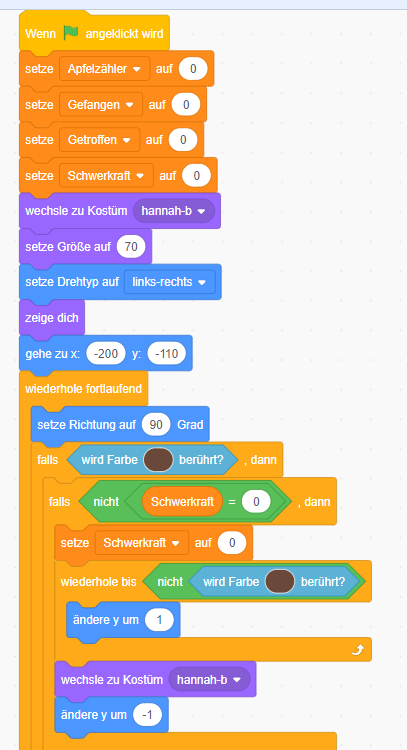
\includegraphics[width=9cm]{FigurenSkript.png}
    \hspace{0.5cm}
    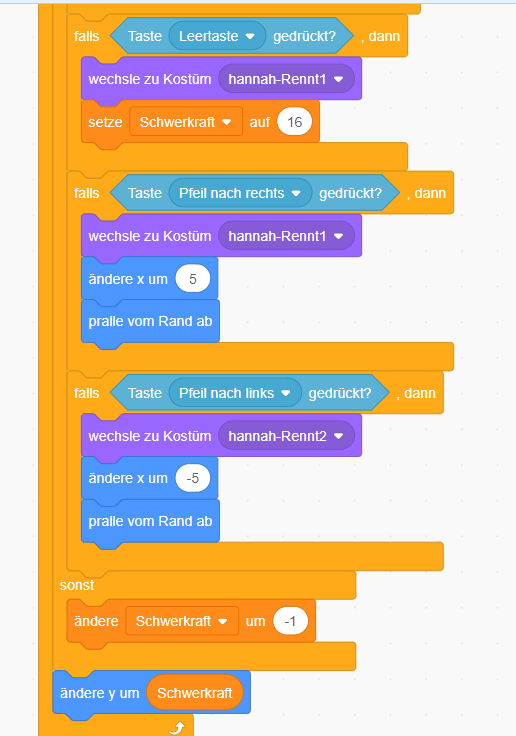
\includegraphics[width=9.25cm]{FigurenSkript2.png}


    \vspace{0.5cm}
    \SectionDesign{subsection}{18}{24}{\textbf{Skript für die Hecke}}
    \vspace{0.25cm}

    \TextDesign{
    Die Hecke bewegt sich fortlaufend von rechts nach links. Dies verleiht dem Spiel eine dynamische Umgebung, in der die Spieler ständig in Bewegung bleiben müssen, um Äpfel zu sammeln und den Vögeln auszuweichen.

    Hier ist, wie die Animation der Hecke funktioniert:
    
    \begin{itemize}
        \item Die Hecke bewegt sich 5 Schritte von rechts nach links fortlaufend.
        \item Sobald die Hecke den linken Rand des Bildschirms erreicht, wird sie wieder an den rechten Rand versetzt.
        \item Es wird ein Klon benötigt, um einen flüssigen Verlauf von den beiden Hecken zu schaffen.
    \end{itemize}
    
    Da die gleichen Blöcke an Code für die Hecke und den Klon verwendet werden, speichern wir diese in unserem eigenen Block \textit{Bewege}, welchen wir mehrfach verwenden können. Dafür drücke auf \textit{Meine Blöcke} an der Seite und dann auf \textit{neuer Block}.
    }

    \centering
    \vspace{1cm}
    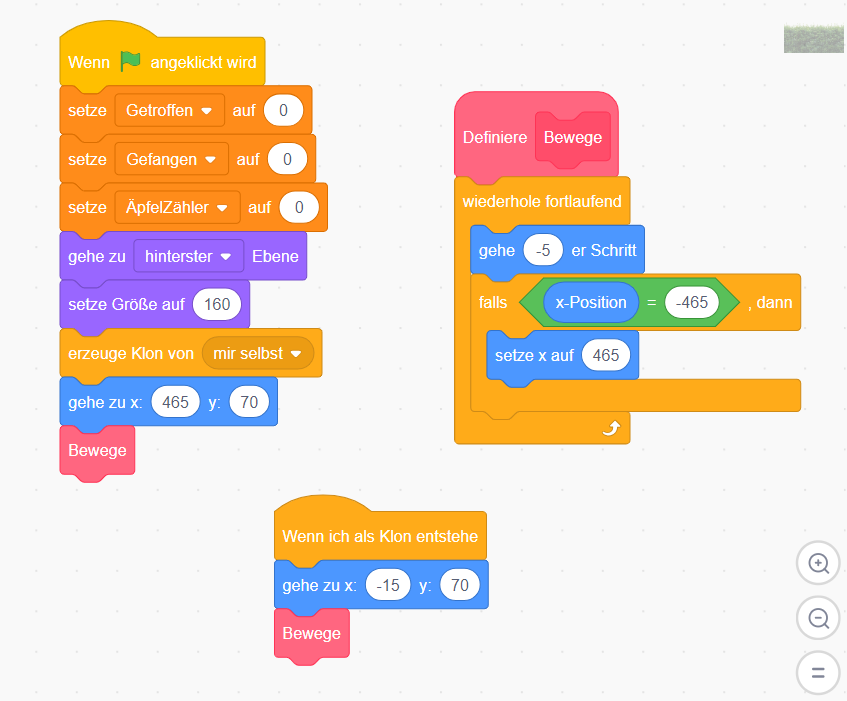
\includegraphics[width=15cm]{HeckeSkript.png}
    \vspace{1cm}

    \RaggedRight
    \SectionDesign{subsection}{18}{24}{\textbf{Skript für Äpfel}}
    \vspace{0.25cm}

    \TextDesign{
    Hier ist, wie das Klonen der Äpfel funktioniert:
    
    \begin{itemize}
        \item Ein ursprünglicher Apfel wird als Vorlage verwendet und an einer zufällig ausgewählten y Position auf der Hecke platziert.
        \item Dieser Apfel wird in regelmäßigen Abständen geklont, sodass immer neue Äpfel erscheinen, die der Spieler einsammeln kann.
        \item Jeder geklonte Apfel bewegt sich mit der Hecke von rechts nach links über den Bildschirm.
        \item Sobald ein Apfel vom Spieler eingesammelt wird oder den linken Rand des Bildschirms erreicht, löscht man den Klon.
        \item der Apfelzähler wird nach jedem geklonten Apfel um 1 erhöht.
    \end{itemize}

    }    

    \centering
    \vspace{1cm}
    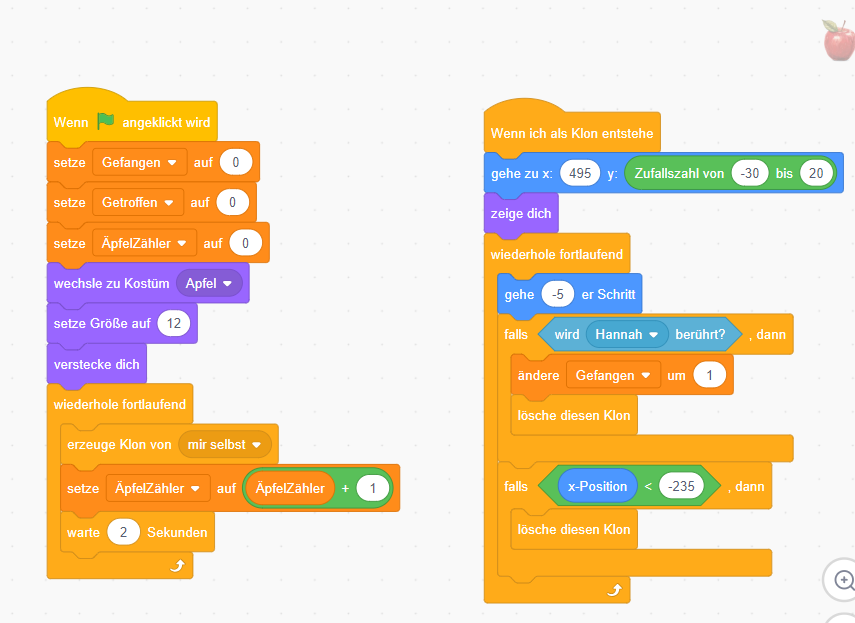
\includegraphics[width=15cm]{ApfelSkript.png}
    \vspace{1cm}

    \RaggedRight
    \SectionDesign{subsection}{18}{24}{\textbf{Skript für Vögel}}
    \vspace{0.25cm}

    \TextDesign{
    Vögel fliegen von rechts nach links über den Bildschirm, um den Spielern zusätzliche Herausforderungen zu bieten. Diese Vögel erscheinen in regelmäßigen Abständen und bewegen sich oberhalb der Hecke.
    
    \begin{itemize}
        \item Ein ursprünglicher Vogel dient als Vorlage und wird regelmäßig an einer zufällig ausgewählten y Position in der Luft geklont.
        \item Jeder Klon startet am rechten Rand des Bildschirms und fliegt von rechts nach links.
        \item Vögel erscheinen in 2 Sekunden Abständen.
        \item Wenn ein Vogel den linken Rand des Bildschirms erreicht oder mit dem Spieler kollidiert, verschwindet er. Dies wird in einem von uns definierten Block \textit{Überprüfe} definiert, da es mehrfach verwendet werden muss.
        \item Jeder Vogel hat eine zufällig ausgewählte Geschwindigkeit und Y Abweichung mit der er nach unten und oben gleiten kann.
        \item Der Vogel wird im Laufe des Spiels schneller und kommt der Figur näher, was in den \textit{wiederhole 25 mal - Schleifen} sichtbar ist. Das macht das Spiel schwieriger und interessanter.
    \end{itemize}

    Durch das clevere Klonen und Platzieren der Vögel wird das Spiel herausfordernder, da die Spieler nicht nur Äpfel sammeln, sondern auch ständig den heranfliegenden Vögeln ausweichen müssen.
    }  

    \centering
    \vspace{1cm}
    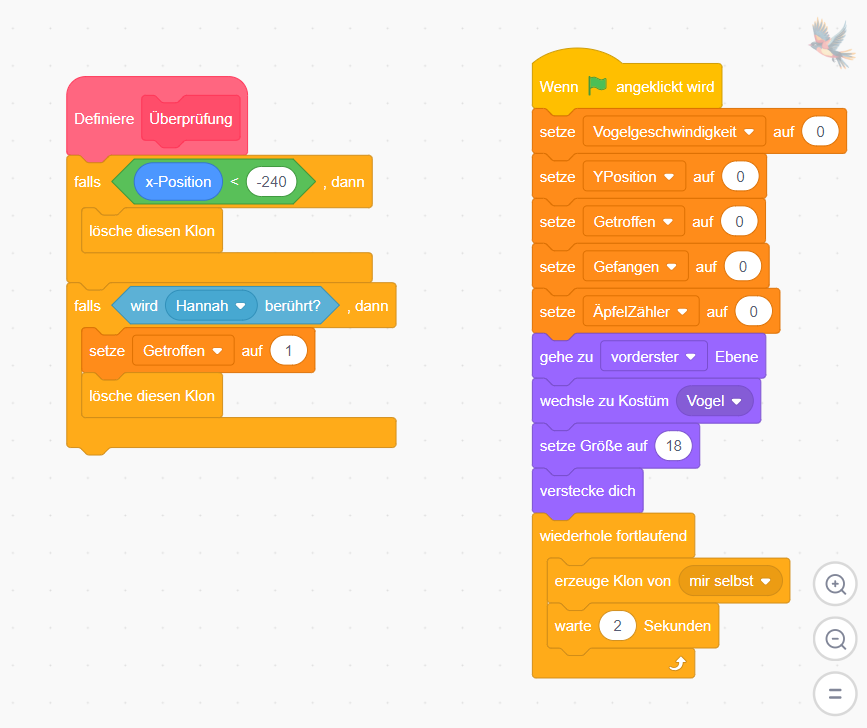
\includegraphics[width=9cm]{VogelSkript.png}
    \hspace{0.5cm}
    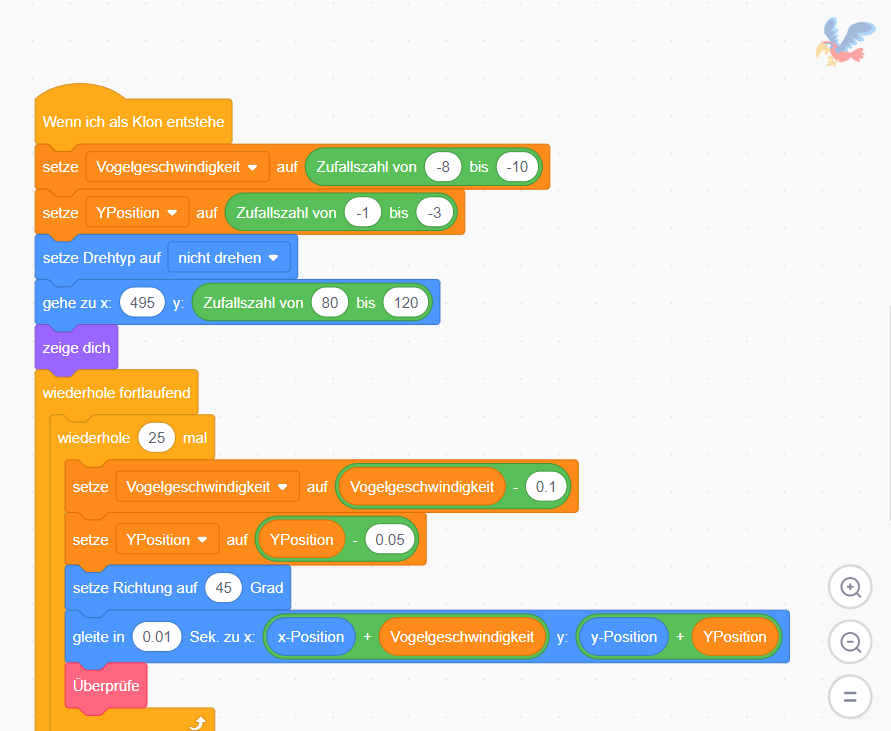
\includegraphics[width=9cm]{VogelSkript2.png}

    \RaggedRight
    \vspace{1cm}
    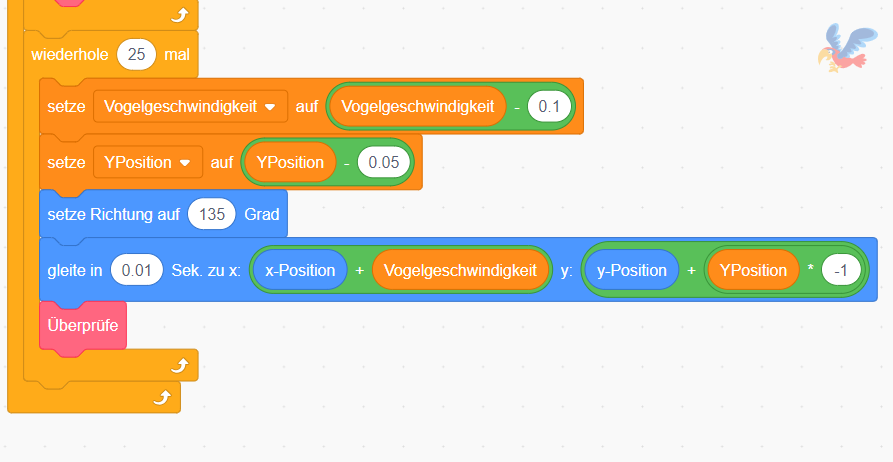
\includegraphics[width=12cm]{VogelSkript3.png}
    \vspace{1cm}

    \SectionDesign{subsection}{18}{24}{\textbf{Letzte Überprüfung}}
    
    \vspace{0.5cm}
    \SectionDesign{subsubsection}{14}{24}{Wechsle zum Kostüm}
    \vspace{0.25cm}

    \TextDesign{
    Der Codeblock wird nur bei der Figur \textit{Vogel} verwendet und überprüft folgende Situationen:

    \begin{itemize}
        \item Wenn die Figur von einem Vogel getroffen wurde,
        \item Wenn die Figur 25 Äpfel gesammelt hat,
        \item Wenn die Figur gar keine Äpfel gesammelt hat und schon 10 Äpfel geklont wurden,
    \end{itemize}

    dann wird die Figur auf die richtige Größe und Position angepasst und gezeigt.
    
    Darunter wird nochmal überprüft ob es sich um \textit{Verloren} oder \textit{Gewonnen} handelt und zum jeweils richtigem Kostüm gewechselt.
    Zuletzt wird das Skript gestoppt.
    }  

    \vspace{0.5cm}
    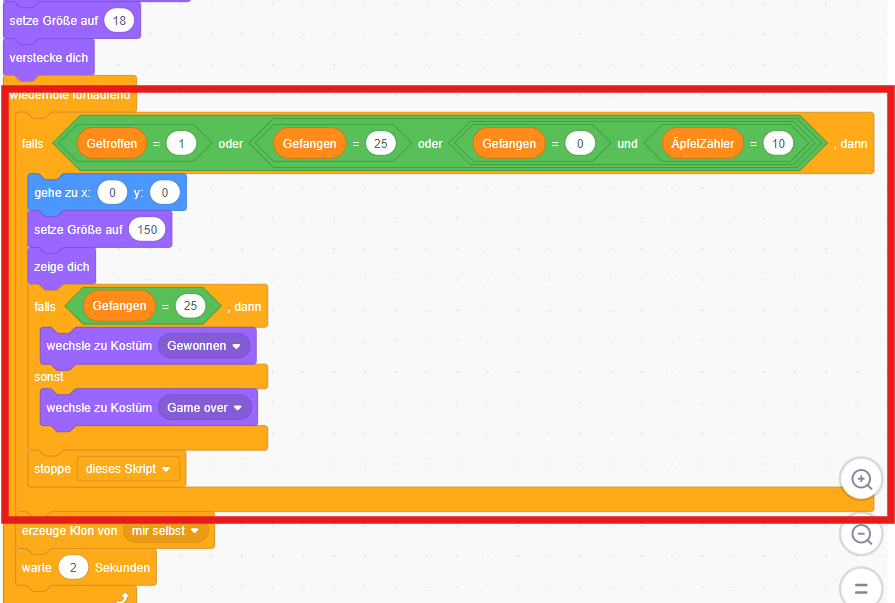
\includegraphics[width=14cm]{VogelÜberprüfung.png}

    \vspace{0.5cm}
    \SectionDesign{subsubsection}{14}{24}{Stoppe dieses Skript}
    \vspace{0.25cm}

    \TextDesign{
    Dieser Codeblock wird bei fast allen Skripts verwendet und überprüft folgende Situationen:

    \begin{itemize}
        \item Wenn die Figur von einem Vogel getroffen wurde,
        \item Wenn die Figur 25 Äpfel gesammelt hat,
        \item Wenn die Figur gar keine Äpfel gesammelt hat und schon 10 Äpfel geklont wurden,
    \end{itemize}

    dann wird das Skript, indem der Codeblock verwendet wird gestoppt.
    }  

    \vspace{0.5cm}
    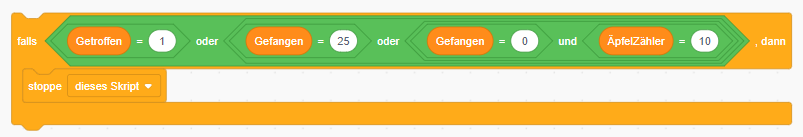
\includegraphics[width=14cm]{Überprüfung.png}
    \vspace{1cm}

    \SectionDesign{subsection}{18}{24}{\textbf{Fertig!}}
    \vspace{0.5cm}

    \TextDesign{
    Gratuliere! Dein Spiel ist fertig. Probiere es gleich aus! Du kannst das fertige Projekt unter \href{https://scratch.mit.edu/projects/1049928428/}{\textcolor{blue}{https://meet.coderdojo.net/\newline scratch-äpfelsammeln}}
    }

    
\end{document}